\chapter{Characterisation of the acousto-optic deflectors}\label{ch:acousto_optic_deflectors}

\textit{In the previous chapter we seeked for different aspects of the
\gls{rf} signal powering the \gls{aod} elements and found that the
electronic equipement provides an overall stable signal for the \gls{aod}.
In this chapter we want to examine the intensity characteristics subject
to frequency and amplitude parameters of the \gls{rf} signal. In the end
we will find that the intensity shows highly non-linear behaviour with
respect to the \gls{rf} signal parameters.}

\section{Difference between individual acousto-optic deflectors}

Our optical setup uses a single two dimensional \gls{aod} that comprises two
\gls{aod} elements perpendicular to each other. At first we want to examine the
behaviour of the individual \gls{aod} elements to each other. In particular we
are interested if and how the elements differ.
\begin{figure}[htb]
  \centering
  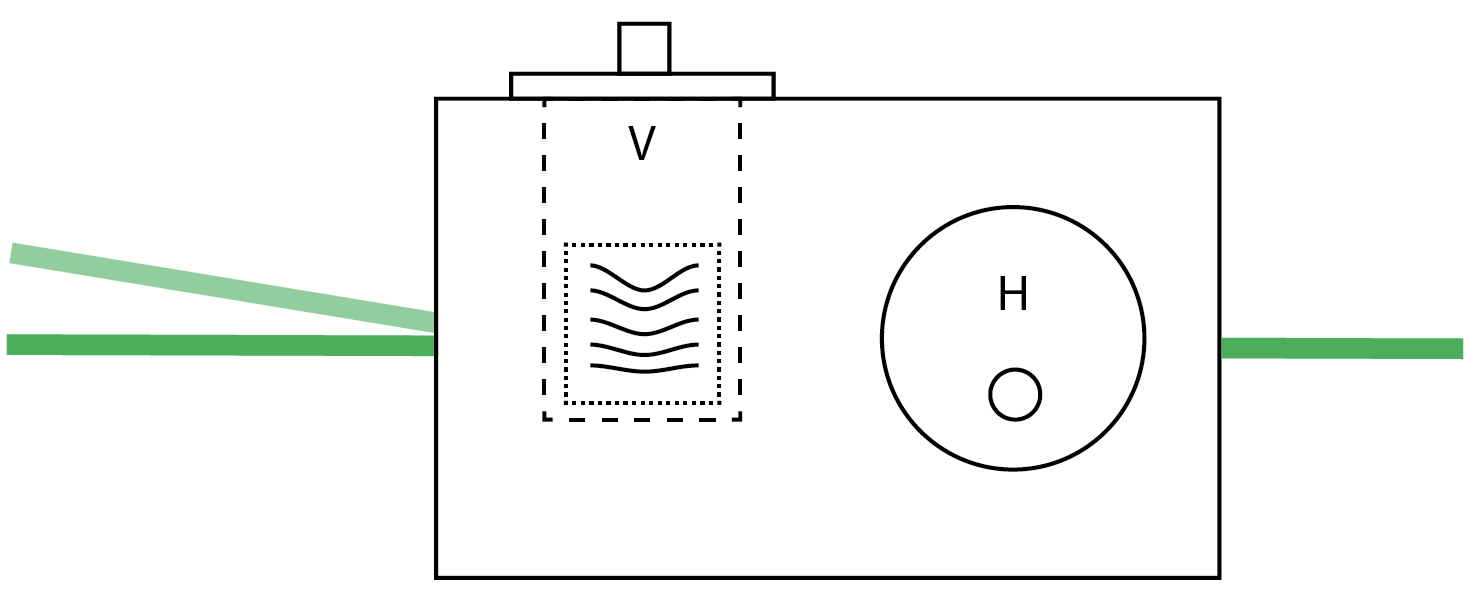
\includegraphics[width=\textwidth]{../media/setup/aod-socket.png}
  \caption{Drawing of the used \gls{2d} \gls{aod}.
  }\label{fig:aod_socket}
\end{figure}
A schematic drawing of the \gls{aod} is depicted in \Cref{fig:aod_socket}. We
see the two \gls{aod} elements in the respective horizontal and vertical slot.
The internals of the vertical \gls{aod} (left-hand side) are illustrated. The
element itself spans through the casing (dashed line) while the acousto-optic
crystal (dotted line) is glued onto the element. The laser beam (green) passes
through the acousto-optic crystal. In the following we will refer to the
horizontal \gls{aod} element as the \gls{aod} element anticipated for the
horizontal slot and accordingly to the vertical \gls{aod} element as the
\gls{aod} element intended for the vertical \gls{aod} socket.

\subsection{Individual acousto-optic deflectors}

For the following experiment we will only leave one \gls{aod} element mounted
in the casing depicted in \Cref{fig:aod_socket}. The other slot will be empty.
Then we will exchange socket positions for each respective \gls{aod} element
and measure the beam intensity subject to the linear frequency sweep from
\SI{80}{\mega\hertz} to \SI{120}{\mega\hertz} over a duration of
\SI{260}{\milli\second} and the configured \gls{dds} amplitude. As \gls{rf}
signal source the amplifier and \gls{dds} combination intended for the
horizontal \gls{aod} element was used to avoid influences of the amplification
offset between the two amplifiers.
\begin{figure}[htb]
  \centering
  \begin{adjustbox}{width=\textwidth}
    \inputpgf{../figure/intensity/distribution}{unpaired-amplitude.pgf}
  \end{adjustbox}
  \caption{Intensity distribution over linear frequency sweep at different
    configured \gls{dds} amplitudes for different individual \gls{aod}
    configurations.
  }\label{fig:intensity_distribution_unpaired}
\end{figure}
The results for the four configurations (horizontal element in horizontal
slot, horizontal element in vertical slot, vertical element in horizontal
slot and vertical element in vertical slot) are visualized as heatmaps in
\Cref{fig:intensity_distribution_unpaired}. The color values are normalized in
between the different heatmaps and can be related to the measured voltage from
the photodiode via the colorbar on the right-hand side. Oddly enough we
observe that both \gls{aod}s differ strongly in their respective intensity
transmission behaviour depending on their slot position. Furthermore we
observe that the intensity transmission is much higher in the case of the
horizontal \gls{aod} element mounted to the intended horizontal slot compared
to all other configurations. In addition we can see that the intensity map
measured with the horizontal \gls{aod} displays a jump. The highest intensity
transmission is obtained for relative amplitudes configured between
\SI{60}{\percent} and \SI{90}{\percent} with large dependence on the
frequency. Another interesting observation is that the intensity transmission
seems very similar for the horizontal element in the vertical slot and the
vertical element in the vertical slot whose map also seems more symmetric with
respect to the frequency axis. In fact for these configurations the amplitude
dependence seems to be essentially independent of the frequency dependence.
We assume that the individual elements are designed for different
polarisation angles. In order to prove this hypothesis we added a tunable
$\lambda/2$ retarder plate after Cube \num{2}. Tuning the $\lambda/2$ retarder
before Cube \num{2} would change the intensity fraction that gets redirected into
the beam dump as Cube \num{2} is a beam splitter sensible to polarisation.
\begin{figure}[htb]
  \centering
  \begin{adjustbox}{width=\textwidth}
    \inputpgf{../figure/intensity/distribution}{polarisation-horizontal.pgf}
  \end{adjustbox}
  \caption{Intensity transmission of the \gls{h} \gls{aod} in the \gls{h} slot
    at maximum output amplitude for different polarisation angles.
  }\label{fig:intensity_polarisation_h}
\end{figure}
In \Cref{fig:intensity_polarisation_h} the intensity transmission of the
\gls{h} \gls{aod} in the \gls{h} slot at maximum output amplitude is presented
for different polarisation angles. The polarisation angles are the remainders
of the angles read of from the retarder plate mount divided by \ang{90}. The
reason behind this step is that a rotation of a retarder plate by $\phi$
effectively changes the polarisation angle by $2\phi$. Further the
polarisation domain is limited to $\left[0,\ang{90}\right]$.
\begin{figure}[htb]
  \centering
  \begin{adjustbox}{width=\textwidth}
    \inputpgf{../figure/intensity/distribution}{polarisation-vertical.pgf}
  \end{adjustbox}
  \caption{Intensity transmission of the \gls{v} \gls{aod} in the \gls{v} slot
    at maximum output amplitude for different polarisation angles.
  }\label{fig:intensity_polarisation_v}
\end{figure}
We note the maximum intensity transmission of the \gls{h} \gls{aod} at
\ang{20} and the minimum intensity transmission at around \ang{70}. The
difference between the polarisation angle at minimum and maximum intensity
is about \ang{50} which is close to \ang{45} that would suggest that
intensity minimum and maximum are located at the respective perpendicular
polarisation axis. In \Cref{fig:intensity_polarisation_v} the intensity
transmission subject to the polarisation angle of the \gls{v} \gls{aod} in
the \gls{v} slot is shown. We again observe a difference of about \ang{45}
between the polarisation angles at maximum and minimum intensity transmission.
\begin{figure}[htb]
  \centering
  \begin{adjustbox}{width=\textwidth}
    \inputpgf{../figure/intensity/distribution}{polarisation.pgf}
  \end{adjustbox}
  \caption{Intensity transmission of the \gls{h} and \gls{v} \gls{aod} at
    \SI{100}{\mega\hertz} and maximum output amplitude for different
    polarisation angles.
  }\label{fig:intensity_polarisation}
\end{figure}
Finally we want to compare the polarisation angles between the individual
\gls{aod}s. Therefore we extracted the intensity transmission at
\SI{100}{\mega\hertz} frequency for both \gls{aod} measurements and plotted
them against the polarisation angle in \Cref{fig:intensity_polarisation}. We
observe a sinusoidal shaped intensity response of the polarisation angle
for the \gls{h} and \gls{v} \gls{aod} which seem out of phase by nearly
\ang{90}.

The \gls{2d} \gls{aod} casing allows to rotate the individual \gls{aod}
elements. So far we choose the rotation angle of the \gls{aod} elements that
maximizes the intensity transmission at the center frequency. What would we
obtain if we tilted the rotation angle a bit to the left and to the right?
\begin{figure}[htb]
  \centering
  \begin{adjustbox}{width=\textwidth}
    \inputpgf{../figure/intensity/distribution}{unpaired-tilted.pgf}
  \end{adjustbox}
  \caption{Intensity distribution at different amplitudes for tilted
    individual \gls{aod}. We observe that the intensity decreases if the
    incident angle deviates from \ang{90}.
  }\label{fig:intensity_distribution_tilted}
\end{figure}
In \Cref{fig:intensity_distribution_tilted} we find the answer to this
question. We observe changes in shape and overall intensity with respect
to the incident angle. We should note that small changes in the incident
angle cause already large deflections of the beam, thus it is not guaranteed
that the left and right measurements are free from aperture effects.
Nevertheless we can record that the incident beam angle is an important
parameter in the intensity transmission of the \gls{aod}s. In particular we
need to consider the incident beam angle for the \gls{2d} \gls{aod}
configuration. It may make sense to change the setup to a configuration
consisting of two \gls{1d} \gls{aod} with a telescope in between.

\section{2D intensity distribution}

In the previous section we sorted out the influence of the \gls{aod} element
position and acknowledged that \gls{aod}s differ significant in their
optical properties. In the present section we now want to explore the
intensity transmission for a two dimensional sweep as intended to be used
for the optical potentials.

The experimental setup is similar to the previous setups and is shown in
\Cref{fig:intensity_distribution_setup}. We have both \gls{aod}s mounted in
their anticipated position. The \gls{aod} elements are aligned to maximize
intensity at the center frequency. The laser beam is directed into a second
photodiode where we measure the intensity with respect to the configured
\gls{dds} signal.
\begin{figure}[htb]
  \centering
  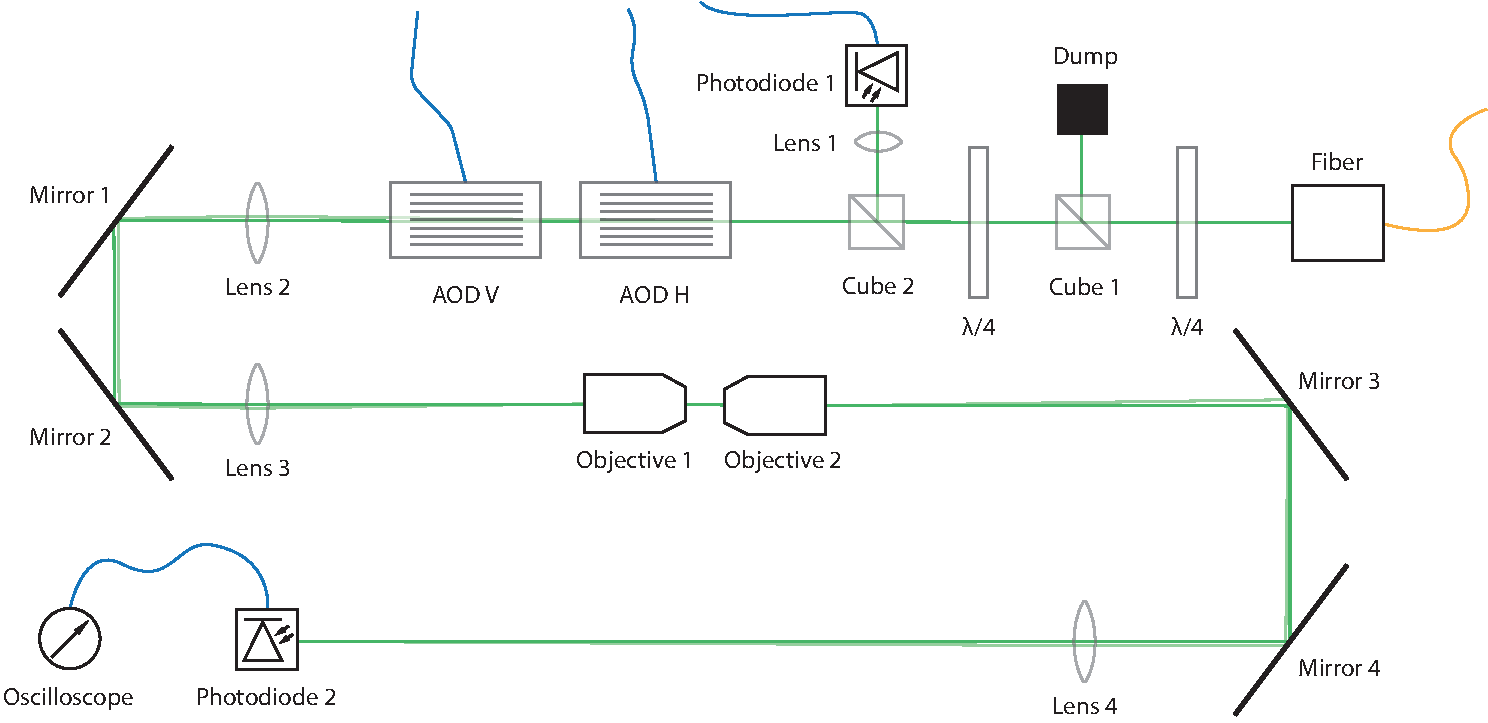
\includegraphics[width=\textwidth]{../media/setup/intensity-distribution.pdf}
  \caption{Experimental setup used to measure the intensity transmission of
    the 2D \gls{aod} in dependence of the configured \gls{dds} signal.
  }\label{fig:intensity_distribution_setup}
\end{figure}

\subsubsection{Digital ramp frequency sweep}

In a first attempt we configure a first \gls{dds} to output a constant
frequency whereas a second \gls{dds} is configured to do a frequency sweep
using the internal digital ramp. After one such sweep the constant frequency
output of the first \gls{dds} is increased and the measurement repeats. The
procedure is repeated until the first \gls{dds} covered the same frequency
range as the second \gls{dds}.
\begin{figure}[htb]
  \centering
  \begin{adjustbox}{width=\textwidth}
    \inputpgf{../figure/intensity/distribution}{paired-frequency.pgf}
  \end{adjustbox}
  \caption{Intensity measured as voltage at the photodiode in dependence of
    the horizontal and vertical applied frequency signal to the \gls{aod}. The
    left map is obtained by enabling the digital ramp on the horizontal
    \gls{dds} whereas the vertical \gls{dds} is configured to output a
    constant frequency which is manually increased after each measurement.
    On the right-hand side map the roles are exchanged.
  }\label{fig:intensity_distribution_frequency}
\end{figure}
In \Cref{fig:intensity_distribution_frequency} we present the intensity
measured at the second photodiode in the setup shown in
\Cref{fig:intensity_distribution_setup}. On the left-hand map the first
\gls{dds} is the \gls{dds} responsible for translations in vertical direction
whereas the second \gls{dds} is responsible for translations in horizontal
direction. The frequency sweep performed by the digital ramp is more dense
compared to the frequency sweep performed by manual increments in our
configuration as the manual increments require driver calls whereas the
digital ramp increments are performed internal of the \gls{dds}.
\begin{figure}[htb]
  \centering
  \begin{adjustbox}{width=\textwidth}
    \inputpgf{../figure/intensity/distribution}{paired-frequency-residue.pgf}
  \end{adjustbox}
  \caption{Absolute difference between the 2D intensity distribution
    performed with the digital ramp configured set to different axes.
  }\label{fig:intensity_distribution_frequency_residue}
\end{figure}
As the differences in \Cref{fig:intensity_distribution_frequency} are of only
subtile nature we additionally reveal the absolute difference between both
maps in \Cref{fig:intensity_distribution_frequency_residue}. We observe
nearly a binary map of dark purple and yellow areas whereas the dark area can
be intepreted as small and the yellow area as large difference. The binary
nature of the absolute difference could be interpreted as a fixed offset
in the power level between the \gls{h} and \gls{v} \gls{rf} signal supplied to
the \gls{aod}s. In areas of small intensity difference (purple) the ouptut
level may be sufficient to saturate the acousto-optics. However we must admit
that these are simply suggestions and need further evidence.

\subsubsection{Constant sampled frequencies}

In \cref{subsec:electronic_amplitude_frequency_response} we did not find
differences in the amplitude frequency response of the amplified \gls{rf}
signal between frequency increments performed by the internal digital ramp of
the \gls{dds} and frequency increments performed by manually updating the
output frequency through the driver. Yet, it remains open if differences
arise in the transmission frequency response of the \gls{aod} as the \gls{aod}
is not a purely electronic device.
\begin{figure}[htb]
  \centering
  \begin{adjustbox}{width=\textwidth}
    \inputpgf{../figure/intensity/distribution}{sample-frequency.pgf}
  \end{adjustbox}
  \caption{Intensity measured as voltage at the photodiode in dependence of
    the horizontal and vertical applied frequency signal to the \gls{aod}.
    Frequency pairs are sampled over a uniform distribution and then passed
    as constant output frequency paramter to the \gls{dds}.
  }\label{fig:intensity_distribution_frequency_sampled}
\end{figure}
To partly answer this question we sampled random frequency pairs over a
two dimensional uniform distribution and passed them as constant frequency
parameter to the respective \gls{dds} through the driver interface. The
yielded intensity distribution is visualized in
\Cref{fig:intensity_distribution_frequency_sampled}. We note that in
comparison to \Cref{fig:intensity_distribution_frequency} the intensity
differences are more concentrated around the vertical axis. We believe that
acousto-optics possess a non-instantaneous frequency response characteristic
that requires further investigation.

\subsubsection{Different radio frequency signal source}

In the previous two sections we found that the \gls{aod}s are quite sensible
to the method used to perform frequency increments in a frequency sweep. In
order to further investigate this phenomena we decided to replace one
\gls{dds} with a high-quality signal generator while the other \gls{dds} was
configured to output a constant \SI{100}{\mega\hertz} signal. The output
level of the signal generator was configured to match the output level of
the \gls{dds} and amplified using the usual power amplifier.
\Cref{fig:intensity_distribution_signal_sources} discloses the different
intensity transmission registered by the photodiode for a frequency sweep
performed by the \gls{dds} through the digital ramp and by the signal
generator. In comparison to the \gls{dds} the signal generator does not
support continous frequency changes as we can see from the intensity drops
between the frequency increments of the signal generator trace.
\begin{figure}[htb]
  \centering
  \begin{adjustbox}{width=\textwidth}
    \inputpgf{../figure/intensity/distribution}{signal-sources.pgf}
  \end{adjustbox}
  \caption{Intensity measured as voltage at the photodiode with one \gls{aod}
    at constant center frequency supplied by a \gls{dds} and the other
    \gls{aod} performing a linear frequency sweep with the \gls{dds} and a
    high-quality signal generator.
  }\label{fig:intensity_distribution_signal_sources}
\end{figure}
Further ignoring these intensity drops we observe that the global response
characteristics differ in particular at the begin of the frequency sweep and
at the center. As the power amplifier remains unchanged through the
measurements and the output voltage of the signal sources are independent of
frequency, we are only left with two explainations. For one the power supplied
to the \gls{aod} could differ as we did not meausre the current response. On
the other the frequency drops in between frequency increments of the signal
generator could cause the observed characteristis. The later hyphothesis would
also confirm the result of the previous section in which we found a different
transmission characteristic for differen frequency sampling strategies.

\subsubsection{Summary}

In summary we found that the intensity transmission of the \gls{aod} show a
highly non-linear dependency in the applied power and the method used for
frequency sampling. It will continue to be interesting to explore the
intensity transmission subject to the effective power of the \gls{rf} signal
applied to the \gls{aod}. So far we only know that the voltage of the \gls{rf}
signal of the \gls{dds} is constant over our frequency range of
\SI{80}{\mega\hertz} to \SI{120}{\mega\hertz}, however we cannot make any
statements with respect to the current characteristics. All in all there are
too many factors to consider to describe with a simple analytical model and we
will further try to work with a model-free optimization procedure in the next
chapter in order to minimize the intensity transmission variance and produce
a constant laser intensity in the atom plane.

\section{Diffraction efficiency optimization}

The previous two chapters addressed the characteristics of the \gls{rf}
signal and the intensity transmission of the \gls{aod}. Therewith the
groundwork has been set out to finally approach the mission of minimizing the
intensity variance to obtain a homogenous optical potential.

But how do we minimize the intensity variance? The \gls{dds} permits to read
$N=1024$ amplitude values from memory. The optimization problem therefore is to
minimize the variance of the intensity distribution $I(A)$ subject to an
amplitude vector $A\in{[0,1]}^N$. The conclusions drawn from the intensity
measurements suggest that we have to expect non-linear, irregular behaviour
in $I(A)$, and indeed first attempts to model $I(A)$ through polynomial fits,
multilayer perceptron networks and least-squared minimizations have failed.

During these optimization procedures we observed that changing an amplitude
value $A_i\in A$ does affect the intensity voltage at subsequent
$A_{i+1},\dots,A_N$. Fortunately we found that by respecting the amplitude
order with respect to increasing frequency during optimization we where able
to bypass these effects. Further we created amplitude segments
$\left(A_j,\dots,A_{j+m}\right)$ consisting of $m$ ordered amplitude values
to reduce the optimization time. Optimization then was performed through
random search which was proven to yield better results as grid
search~\cite{Bergstra2012}.

\subsubsection{Overview}

First, we want to provide an overview of the final optimization results
obtained at different hyperparameters for the random search. The
hyperparameter includes the number of amplitude segments $N/m$ and the target
intensity.
\begin{figure}[htb]
  \centering
  \begin{adjustbox}{width=\textwidth}
    \inputpgf{../figure/intensity/optimization}{overview.pgf}
  \end{adjustbox}
  \caption{Minimized intensity variance for different target intensities
    and number of amplitude segments. We note heavy oscillations for
    amplitude segments greater than eight.
  }\label{fig:intensity_optimization_overview}
\end{figure}
In \Cref{fig:intensity_optimization_overview} we present the final
optimization results for target intensities of \SI{800}{\milli\volt},
\SI{1000}{\milli\volt} and \SI{1200}{\milli\volt} and amplitude segments
$8,16,32$. We observe heavy oscillations for amplitude segments greater than
eight. The optimization results using \num{16} amplitude segments performs
better than the run with \num{32} amplitude segments.

We assume that inductive effects occur when choosing more amplitude segments
that consolidate a non-linear intensity response. For the sake of simplicity
we will first limit us to the case of eight amplitude segments.
\begin{figure}[htb]
  \centering
  \begin{adjustbox}{width=\textwidth}
    \inputpgf{../figure/intensity/optimization}{intensity-amplitude.pgf}
  \end{adjustbox}
  \caption{Final result of the intensity variance minimization and the
    corresponding amplitude segment values obtained through random search with
    eight independent amplitude segments.
  }\label{fig:intensity_optimization_intensity_amplitude}
\end{figure}
In \Cref{fig:intensity_optimization_intensity_amplitude} we have a closer
view on the first column of \Cref{fig:intensity_optimization_overview}. We
can notice similar characteristics observed in the \gls{rf} signal. In
particular the more power drop near the center frequency is present and the
linear power fall off with the frequency in the second half of the frequency
sweep.

\subsubsection{Process}

We now want to elaborate on the optimization process. We limit ourselves to
the optimization process with eight amplitude segments as it was the most
successful one and can be covered completly with eight plots.
\begin{figure}[htb]
  \centering
  \begin{adjustbox}{width=\textwidth}
    \inputpgf{../figure/intensity/optimization}{process.pgf}
  \end{adjustbox}
  \caption{Intensity and amplitude at different stages of the optimization
    process. In each column a different amplitude segment is optimized.
    The different traces in each plot mark the respective iteration.
  }\label{fig:intensity_optimization_process}
\end{figure}
In \Cref{fig:intensity_optimization_process} we see the intensity and
amplitude at different optimization stages. At each stage one amplitude
segment is sampled from a uniform distribution over $[0.2,0.8]$. The intensity
segment associated with this amplitude segment is then used to calculate
the \gls{mse} and compare it to the previous best \gls{mse}. If the new
\gls{mse} is less than the previous best \gls{mse} the previous best \gls{mse}
is updated and the amplitude segment value is saved. This procedure is
repeated \num{500} times. Every time a new best value was found we saved the
data. For the diagrams we choose the four most separated iteration steps to
visualize the process of the optimization.

If we take a look at the succeeding segment from the currently optimized
amplitude segment we observe that these differ for different amplitude
values and henceforth confirms that amplitude values are not independent but
affect subsequent segments.

\subsubsection{Failure}

With the optimization showing reasonable convergence for eight amplitude
segments we would expect it to improve if we choose a more amplitude segments,
yet we observed heavy oscillations. In this section we want to check the
optimization process in the case of \num{32} amplitude segments to investigate
in possible origins of the optimization failure.
\begin{figure}[htb]
  \centering
  \begin{adjustbox}{width=\textwidth}
    \inputpgf{../figure/intensity/optimization}{failure.pgf}
  \end{adjustbox}
  \caption{Optimization progress for the 2.,4.,6.,8.,10.\ and 20.\ amplitude
    segment of the failed optimization run with 32 amplitude segments. We can
    see that with increasing amplitude segments the non-linear response
    following the optimized amplitude segment increases.
  }\label{fig:intensity_optimization_failure}
\end{figure}
In \Cref{fig:intensity_optimization_failure} we can see the optimization
progress for selected amplitude segments of the optimization run with 32
segments. We observe that with the non-linear response following the actual
optimized amplitude segment increases more and more.

\subsubsection{Summary}

Our attemps to minimize the intensity variance where of mixed success. One
the one hand side we were able to minimize the intensity deviation down
to \SI{100}{\milli\volt} on the other hand we were not able to train any
model on the intensity response that would allow fast optimization or even
predicition of the expected intensity response given an amplitude
configuration.

However we also found out that irregularities arise with increase in the
number of amplitude segments. We suspect that fast changes of the output
amplitude draws power that may non deterministicyl affect the next clock
cycle inside the \gls{dds}. Given that the one dimensional optimizations
already required multiple hours to run and the non-linear response between
amplitude segments we do not believe that it is not in the capabilites of the
\gls{dds} to compensate for the two dimensional intensity distribution
measured in the previous chapter.
\chapter{Intensity transmission optimization}

The previous two chapters addressed the characteristics of the \gls{rf}
signal and the intensity transmission of the \gls{aod}. Therewith the
groundwork has been set out to finally approach the mission of minimizing the
intensity variance to obtain a homogenous optical potential.

But how do we minimize the intensity variance? The \gls{dds} permits to read
$N=1024$ amplitude values from memory. The optimization problem therefore is to
minimize the variance of the intensity distribution $I(A)$ subject to an
amplitude vector $A\in{[0,1]}^N$. The conclusions drawn from the intensity
measurements suggest that we have to expect non-linear, irregular behaviour
in $I(A)$, and indeed first attempts to model $I(A)$ through polynomial fits,
multilayer perceptron networks and least-squared minimizations have failed.

During these optimization procedures we observed that changing an amplitude
value $A_i\in A$ does affect the intensity voltage at subsequent
$A_{i+1},\dots,A_N$. Fortunately we found that by respecting the amplitude
order with respect to increasing frequency during optimization we where able
to bypass these effects. Further we created amplitude segments
$\left(A_j,\dots,A_{j+m}\right)$ consisting of $m$ ordered amplitude values
to reduce the optimization time. Optimization then was performed through
random search which was proven to yield better results as grid
search~\cite{Bergstra2012}.

\subsubsection{Overview}

First, we want to provide an overview of the final optimization results
obtained at different hyperparameters for the random search. The
hyperparameter includes the number of amplitude segments $N/m$ and the target
intensity.
\begin{figure}[htb]
  \centering
  \begin{adjustbox}{width=\textwidth}
    \inputpgf{../figure/intensity/optimization}{overview.pgf}
  \end{adjustbox}
  \caption{Minimized intensity variance for different target intensities
    and number of amplitude segments. We note heavy oscillations for
    amplitude segments greater than eight.
  }\label{fig:intensity_optimization_overview}
\end{figure}
In \Cref{fig:intensity_optimization_overview} we present the final
optimization results for target intensities of \SI{800}{\milli\volt},
\SI{1000}{\milli\volt} and \SI{1200}{\milli\volt} and amplitude segments
$8,16,32$. We observe heavy oscillations for amplitude segments greater than
eight. The optimization results using \num{16} amplitude segments performs
better than the run with \num{32} amplitude segments.

We assume that inductive effects occur when choosing more amplitude segments
that consolidate a non-linear intensity response. For the sake of simplicity
we will first limit us to the case of eight amplitude segments.
\begin{figure}[htb]
  \centering
  \begin{adjustbox}{width=\textwidth}
    \inputpgf{../figure/intensity/optimization}{intensity-amplitude.pgf}
  \end{adjustbox}
  \caption{Final result of the intensity variance minimization and the
    corresponding amplitude segment values obtained through random search with
    eight independent amplitude segments.
  }\label{fig:intensity_optimization_intensity_amplitude}
\end{figure}
In \Cref{fig:intensity_optimization_intensity_amplitude} we have a closer
view on the first column of \Cref{fig:intensity_optimization_overview}. We
can notice similar characteristics observed in the \gls{rf} signal. In
particular the more power drop near the center frequency is present and the
linear power fall off with the frequency in the second half of the frequency
sweep.

\subsubsection{Process}

We now want to elaborate on the optimization process. We limit ourselves to
the optimization process with eight amplitude segments as it was the most
successful one and can be covered completly with eight plots.
\begin{figure}[htb]
  \centering
  \begin{adjustbox}{width=\textwidth}
  %  \inputpgf{../figure/intensity/optimization}{process.pgf}
  \end{adjustbox}
  \caption{Intensity and amplitude at different stages of the optimization
    process. In each column a different amplitude segment is optimized.
    The different traces in each plot mark the respective iteration.
  }\label{fig:intensity_optimization_process}
\end{figure}
In \Cref{fig:intensity_optimization_process} we see the intensity and
amplitude at different optimization stages. At each stage one amplitude
segment is sampled from a uniform distribution over $[0.2,0.8]$. The intensity
segment associated with this amplitude segment is then used to calculate
the \gls{mse} and compare it to the previous best \gls{mse}. If the new
\gls{mse} is less than the previous best \gls{mse} the previous best \gls{mse}
is updated and the amplitude segment value is saved. This procedure is
repeated \num{500} times. Every time a new best value was found we saved the
data. For the diagrams we choose the four most separated iteration steps to
visualize the process of the optimization.

If we take a look at the succeeding segment from the currently optimized
amplitude segment we observe that these differ for different amplitude
values and henceforth confirms that amplitude values are not independent but
affect subsequent segments.

\subsubsection{Failure}

With the optimization showing reasonable convergence for eight amplitude
segments we would expect it to improve if we choose a more amplitude segments,
yet we observed heavy oscillations. In this section we want to check the
optimization process in the case of \num{32} amplitude segments to investigate
in possible origins of the optimization failure.
\begin{figure}[htb]
  \centering
  \begin{adjustbox}{width=\textwidth}
    \inputpgf{../figure/intensity/optimization}{failure.pgf}
  \end{adjustbox}
  \caption{Optimization progress for the 2.,4.,6.,8.,10.\ and 20.\ amplitude
    segment of the failed optimization run with \num{32} amplitude segments.
    We can see that with increasing amplitude segments the non-linear response
    following the optimized amplitude segment increases.
  }\label{fig:intensity_optimization_failure}
\end{figure}
In \Cref{fig:intensity_optimization_failure} we can see the optimization
progress for selected amplitude segments of the optimization run with 32
segments. We observe that with the non-linear response following the actual
optimized amplitude segment increases more and more.

\subsubsection{Summary}

Our attemps to minimize the intensity variance where of mixed success. One
the one hand side we were able to minimize the intensity deviation down
to \SI{100}{\milli\volt} on the other hand we were not able to train any
model on the intensity response that would allow fast optimization or even
predicition of the expected intensity response given an amplitude
configuration.

However we also found out that irregularities arise with increase in the
number of amplitude segments. We suspect that fast changes of the output
amplitude draws power that may non deterministicly affect the next clock
cycle inside the \gls{dds}. Given that the one dimensional optimizations
already required multiple hours to run and the non-linear response between
amplitude segments we do not believe that it is not in the capabilites of the
\gls{dds} to compensate for the two dimensional intensity distribution
measured in the previous chapter.
